\documentclass[12pt]{article}
\usepackage[utf8]{inputenc}
\usepackage[spanish]{babel}
\usepackage[top=2.5cm, bottom=2.5cm, left=2.2cm, right=2.2cm]{geometry}
\usepackage{amsmath}
\usepackage{amsfonts}
\usepackage{caption}
\usepackage{amssymb}
\usepackage{graphicx}
\usepackage{placeins}
\usepackage{float}
\usepackage{subfig}
\usepackage{listings}
\usepackage{grffile}
%\usepackage{pgfplots}


\begin{document}
\renewcommand{\listtablename}{Índice de tablas} 
\renewcommand{\tablename}{Tabla} 


\title{Objetos astrofísicos: Parcial 2}
\author{
Andrés Antonio Fernández \\
Johan Sammir Mendez \\
Edisson Leonardo Peralta
}
\maketitle

\section{Resumen}
En el presente trabajo se hará el análisis estructural para 3 estrellas de 0.45, 7.5 y 52 masas solares gracias a la interpolación realizada a partir de los datos proporcionados en la (figura \ref{fig:zams}). Dicha interpolación se hizo por medio del método llamado "interpolación cubica de hermite".
 Posteriormente los valores obtenidos se ingresaron en el código fuente de \textit{FORTRAN} con el nombre \textbf{zams.for} y de esta manera tener los algunos datos que nos permitieran hacer el respectivo análisis estructural. A continuación se procedió a realizar una serie de gráficas que nos permitieran ver de manera mas clara la estructura de las estrellas en cuestión. Una vez obtenidas las gráficas se procedió a realizar un análisis de éstas. 

\section{Introducción}


\begin{figure}[H]
    \centering   
    \includegraphics[width=0.7\textwidth,angle =-90 ]{tablazams.pdf}
    \caption{Tabla de modelos ZAMS.}
    \label{fig:zams}
\end{figure}


\section{Procedimiento y métodos}
Se desea obtener modelos teóricos para estrellas con 0.45, 7.5 y 52 veces la masa del sol. Ya que éstos datos no están en la figura \ref{fig:zams}, es necesario interpolar los valores de las demás variables.

Para escoger el mejor método, a continuación se mostrara una serie de comparaciones de los resultados obtenidos al aplicar algunas técnicas de ajuste de curvas.

Inicialmente se realizara la gráfica de $log(L/L_s)$ contra $M/M_s$, la cual se puede ver en la figura \ref{fig:dats}. Como se puede apreciar, los puntos poseen una distribución exponencial, por lo que un método de ajuste válido sería un ajuste exponencial. 

En la figura \ref{fig:power} se muestra dicho ajuste, la función obtenida esta dada por la ecuación \ref{eq:power}.
\begin{equation}
 f(x) = a \cdot x^b+c
\label{eq:power}
\end{equation}
Donde $a = -68.57$, $b = -0.02237$ y $c = 68.65$.

\begin{figure}[H]
    \centering   
    \includegraphics[width=0.8\textwidth]{dats.eps}
    \caption{Puntos de la curva $log(L/L_s)$ contra $M/M_s$.}
    \label{fig:dats}
\end{figure}

\begin{figure}[H]
    \centering   
    \includegraphics[width=0.8\textwidth]{power.eps}
    \caption{Ajuste exponencial de la curva.}
    \label{fig:power}
\end{figure}

Éste ajuste sería válido en algunos contextos pero en este caso una interpolación ideal debería seguir la forma de los datos de una forma mas exacta. Para éstos casos una alternativa es usar un método alternativo llamado \textit{"Piecewise Cubic Hermite Interpolating Polynomial"} \cite{NM}, el cual está disponible en el software \textit{Matlab}. Dicho método tiene el beneficio de conservar o seguir de forma mas exactas los datos, es decir, crea funciones monótonas (también llamadas isótonas) ya que estos datos, si bien tienen un comportamiento exponencial aproximado, su forma es más monótona \cite{PCHIP}.

La comparación de el ajuste exponencial con la interpolación cubica de Hermite se muestra en la figura \ref{fig:PCHIP}.

\begin{figure}[H]
    \centering   
    \includegraphics[width=1\textwidth]{PCHIP.eps}
    \caption{Ajuste exponencial contra interpolación cúbica de Hermite.}
    \label{fig:PCHIP}
\end{figure}

En la anterior figura es claro que el segundo método se ajusta mejor a los datos. Incluso, por lo mostrado, es de esperar que el método de interpolación cubica de Hermite proporcione mejores curvas incluso para distribuciones mas complejas de datos.
Por lo tanto es el método que se usará para obtener las variables necesarias para la realización de los modelos de las estrellas propuestas.

Para el cálculo de los modelos se usará el código fuente de \textit{FORTRAN} con el nombre de \textbf{zams.for}. En la tabla \ref{tab:data}.

\begin{table}[H]
\centering
\begin{tabular}{|c|c|c|c|c|c|c|}
\hline  
M/Ms   & X    & Y    & Pc        & Tc           & R               & L/Ls           \\ \hline
0.45   & 0.7  & 0.28 & 1.1729e17 & 8.62914224e6 & 3.12182635e10   & 0.0267908687   \\ \hline
7.5    & 0.74 & 0.24 & 4.8187e16 & 28.8104044e6 & 21.8680933e10   & 2346.2918      \\ \hline
52     & 0.74 & 0.24 & 1.7108e16 & 38.7331329e6 & 65.7168164e10   & 386007.399     \\ \hline
\end{tabular}
\caption{Valores interpolados para las estrellas propuestas}
\label{tab:data}
\end{table}


\section{Análisis}

Si la masa del sistema ZAMS es está especificada las ecuaciones de estructura estelar se pueden resolver y para tal solución obtenemos información acerca de las siguientes cantidades en función del radio (Radio total R, Luminosidad L , Temperatura T  y presión P). Se muestran los resultados para cada una de las estrellas asignadas

%% Para un estudio completo de las estrellas se requiere modelar diferentes estados evolución. Para empezar con este propósito se debe entender como los cuerpos aislados de cierta masa , en este caso las correspondientes a $0.45M_{\odot},7.5M_{\odot},52M_{\odot}$ y su composición química determinan la estructura interna del objeto astronómico. Para poder entender tal proceso se hace necesario plantear modelos de como se genera la energía, cómo se transporta y la naturaleza del equilibrio hisdrostático.

%% Vamos a empezar la discusión considerando que las estrellas tienen simetría esférica y además se encuentran en estado estacionario en donde las variables físicas dependerán exclusivamente de la componente radial, bajo esta aproximación. La ecuación del equilibrio hidrostático del modelo es la siguiente

\begin{eqnarray}
	\frac{dP}{dr} = -G\frac{M(r)\rho(r)}{r^2}
\end{eqnarray}

donde $M(r)$ y $\rho(r)$ describen la masa y la densidad, respectivamente en una esfera de radio r. Esto se expresa de la siguiente manera

\begin{eqnarray}
	\frac{dM(r)}{dr} = 4\pi r^2 \rho
\end{eqnarray}

Las anteriores ecuaciones están conectadas a través de tres variables, la presión, la densidad y la masa, se necesita encontrar una ecuación adicional para tener un sistema cerrado, en este caso se considera un fluido baritrópico , en el cual la presión solamente es función de la densidad




A continuación veremos las gráficas obtenidas a partir del modelo. Ademas  haremos un análisis de estas. 

\begin{figure}[H]
    \centering   
    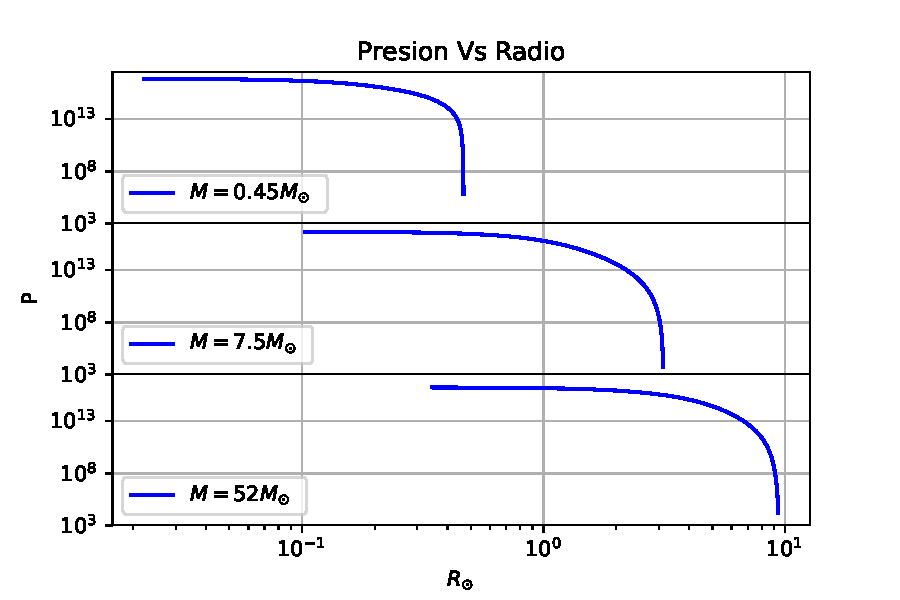
\includegraphics[width=0.9\textwidth]{Presion_graficas.pdf}
    \caption{Perfil obtenido de la presión para cada una de las estrellas en consideración, datos obtenidos en }
    \label{fig:zams}
\end{figure}


Para la masa descrita en la supuesta esfera, se tiene que preservar la masa, 

\newpage


\begin{figure}[H]
    \centering   
    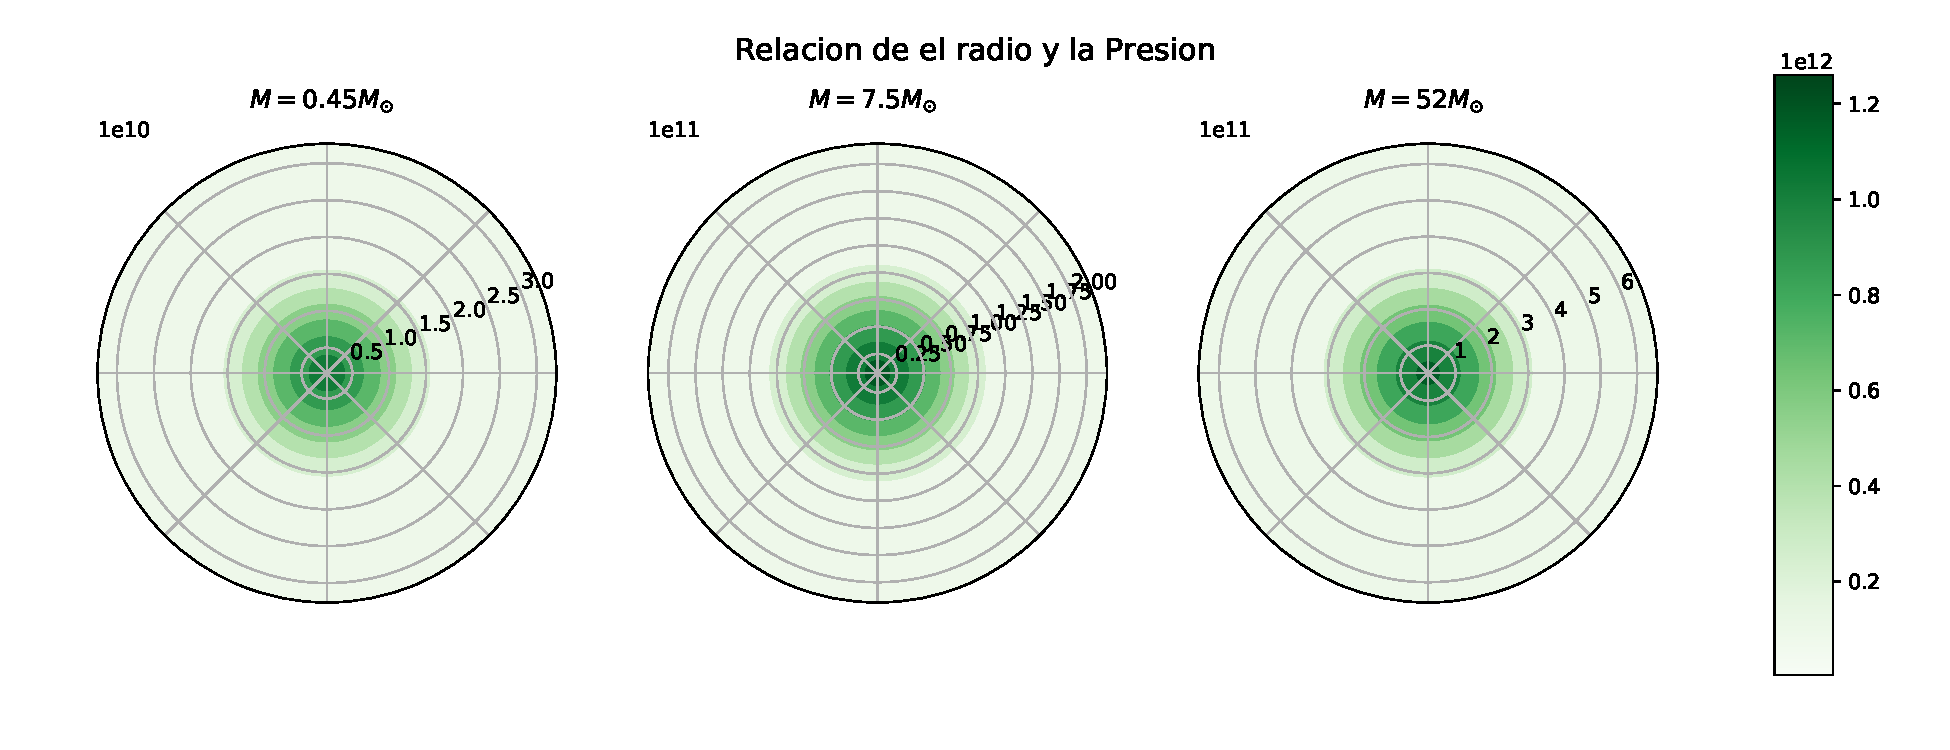
\includegraphics[width=1.0\textwidth]{Polar_presion.pdf}
    \caption{Tabla de modelos ZAMS.}
    \label{fig:zams}
\end{figure}





Observando y analizando las figuras 5, 6 y 7 podemos apreciar que tienen un comportamiento similar, mientras menor es el radio la presión es mayor y mientras mayor es el radio la presión es menor. Esta tendencia se debe a que el centro de la estrella es el punto de mayor presión, ya que soporta el peso de toda la masa. Por otra parte se tiene que es la región donde el ritmo de reacciones de fusión es más elevado.





Al observar las figuras 8, 9 y 10 vemos que la relación entre la densidad y el radio es proporcional en las 3 estrellas analizadas. Esto se debe principalmente a que existe una dependencia entre la presión y al densidad, si la presión es mayor también lo será la densidad.
Por otra parte vemos que para la estrella de menor masa $(0.45)$ la densidad disminuye mas lentamente que para la estrella de mayor masa $(52)$. La razón es que como pudimos ver anteriormente para la presión esto también ocurre.  

\begin{figure}[H]
    \centering   
    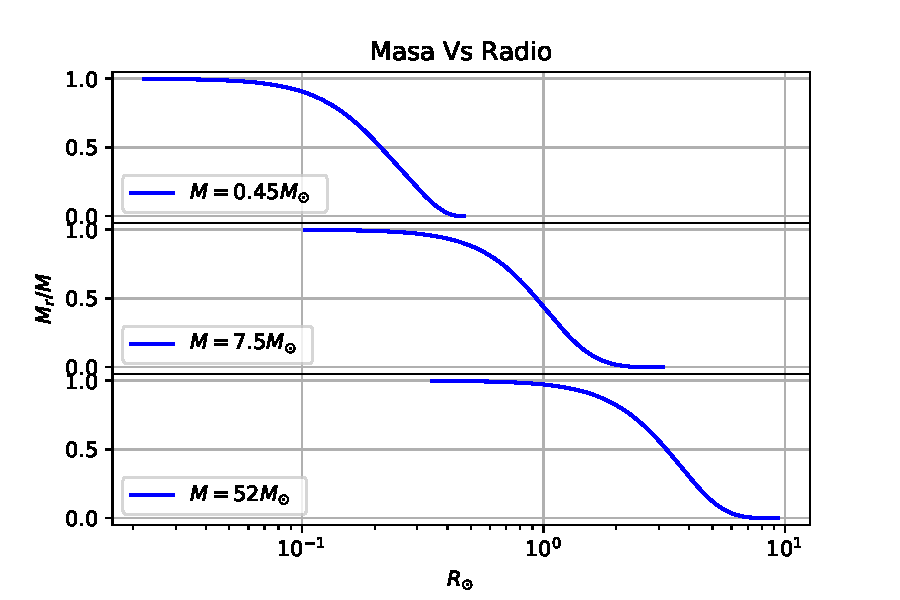
\includegraphics[width=0.8\textwidth]{Masa_graficas.pdf}
    \caption{Tabla de modelos ZAMS.}
    \label{fig:zams}
\end{figure}


Como podemos observar para las figuras 11, 12 y 13 se obtiene tiene el mismo comportamiento. La masa en una estrella esta definida como :

\begin{equation}
M(r)=\int_{0}^{r}  \! \rho (r) 4\pi r^2 \, dr .
\end{equation}

Vemos que depende de la densidad y el radio, de manera que no es de extrañarnos que disminuya o aumente de la una manera similar a como lo hace la densidad en función del radio. \cite{AE}  


\begin{figure}[H]
    \centering   
    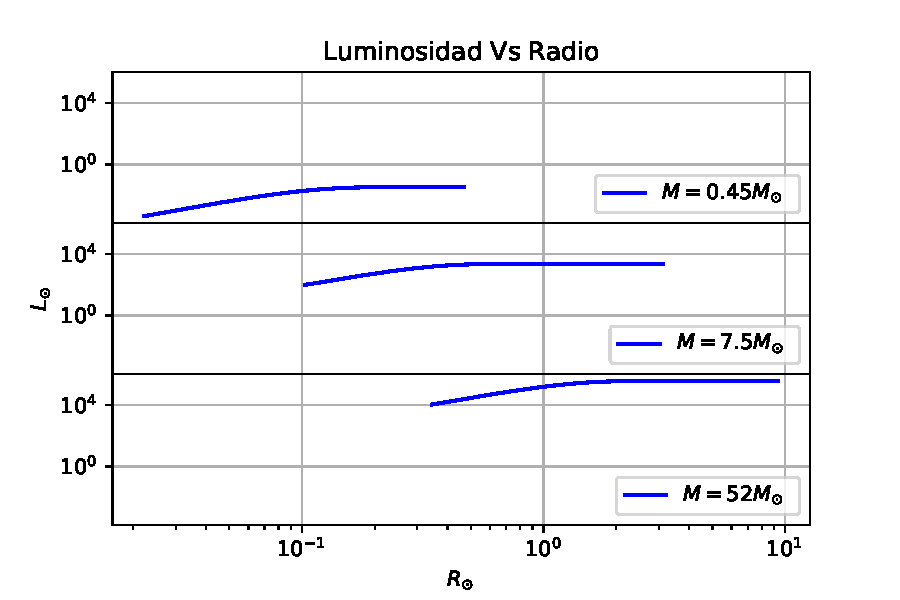
\includegraphics[width=0.8\textwidth]{Luminosidad_graficas.pdf}
    \caption{Tabla de modelos ZAMS.}
    \label{fig:zams}
\end{figure}


La luminosidad de una estrella ($L_r$) es el flujo de la energía que se genera en el centro por las reacciones de fusión y es transportada hacia la superficie. Esta se define de la siguiente manera:

\begin{equation}
\frac{dL_r}{dr} = 4 \pi r^2 \rho \epsilon 
\end{equation}

donde $\epsilon$ es la tasa de generación de energía por unidad masa y es una función conocida de $\rho$, $T$, y la composición química, que se obtiene de la física nuclear. Al igual que en las gráficas anteriores vemos que la luminosidad aumenta o disminuye acorde al radio de la estrella. \cite{AE}
 

\begin{figure}[H]
    \centering   
    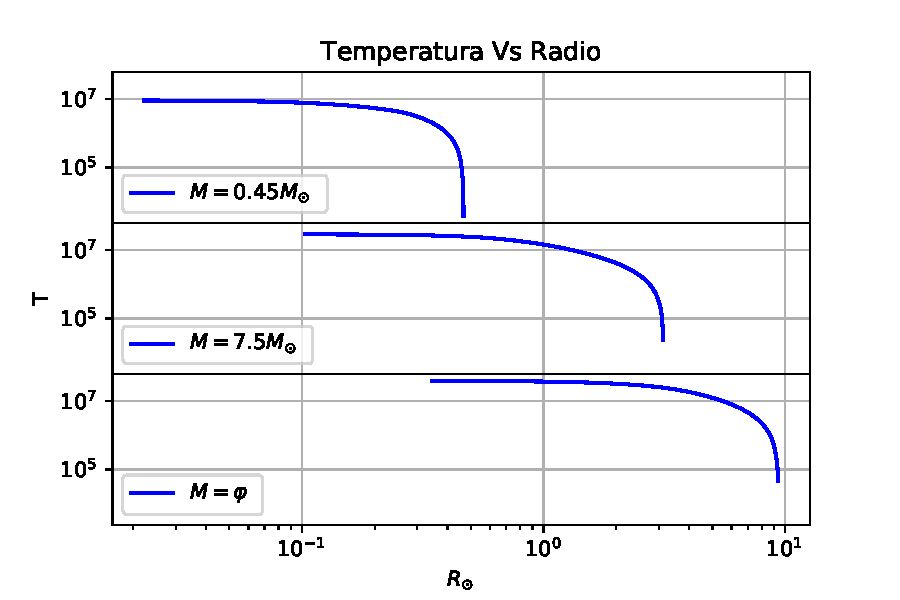
\includegraphics[width=0.8\textwidth]{Temperatura_graficas.pdf}
    \caption{Tabla de modelos ZAMS.}
    \label{fig:zams}
\end{figure}



Finalmente vemos que la temperatura aumenta o disminuye de acuerdo al radio, esto se debe a que como vimos anteriormente en el centro de la estrella es donde ocurren la mayor cantidad de fusiones nucleares haciendo que la temperatura en esta zona sea muy elevada. A medida que el radio se hace mayor las fusiones nucleares disminuyen y por ende la temperatura también se hace cada vez menor tal y como lo vemos en las figuras 16, 17 y 18.



\begin{thebibliography}{10}

\bibitem{NM}
 Kahaner, David, Cleve Moler, Stephen Nash. 
\newblock Numerical Methods and Software.
\newblock Upper Saddle River, NJ: Prentice Hall, 1988.

\bibitem{PCHIP}
 Fritsch, F. N. and R. E. Carlson.
\newblock Monotone Piecewise Cubic Interpolation.
\newblock {SIAM Journal on Numerical Analysis.} Vol. 17, 1980, pp.238–246.

\bibitem{AE}
S. J. Arthur,  Centro de Radioastronomía y Astrofísica, UNAM. 
\newblock Astrofísica Estelar.
\newblock {4 de abril de 2012}.






\end{thebibliography}
\end{document}
